\section{System Demonstration}
\label{sec-demo}

\begin{figure*}[tp]
\centering
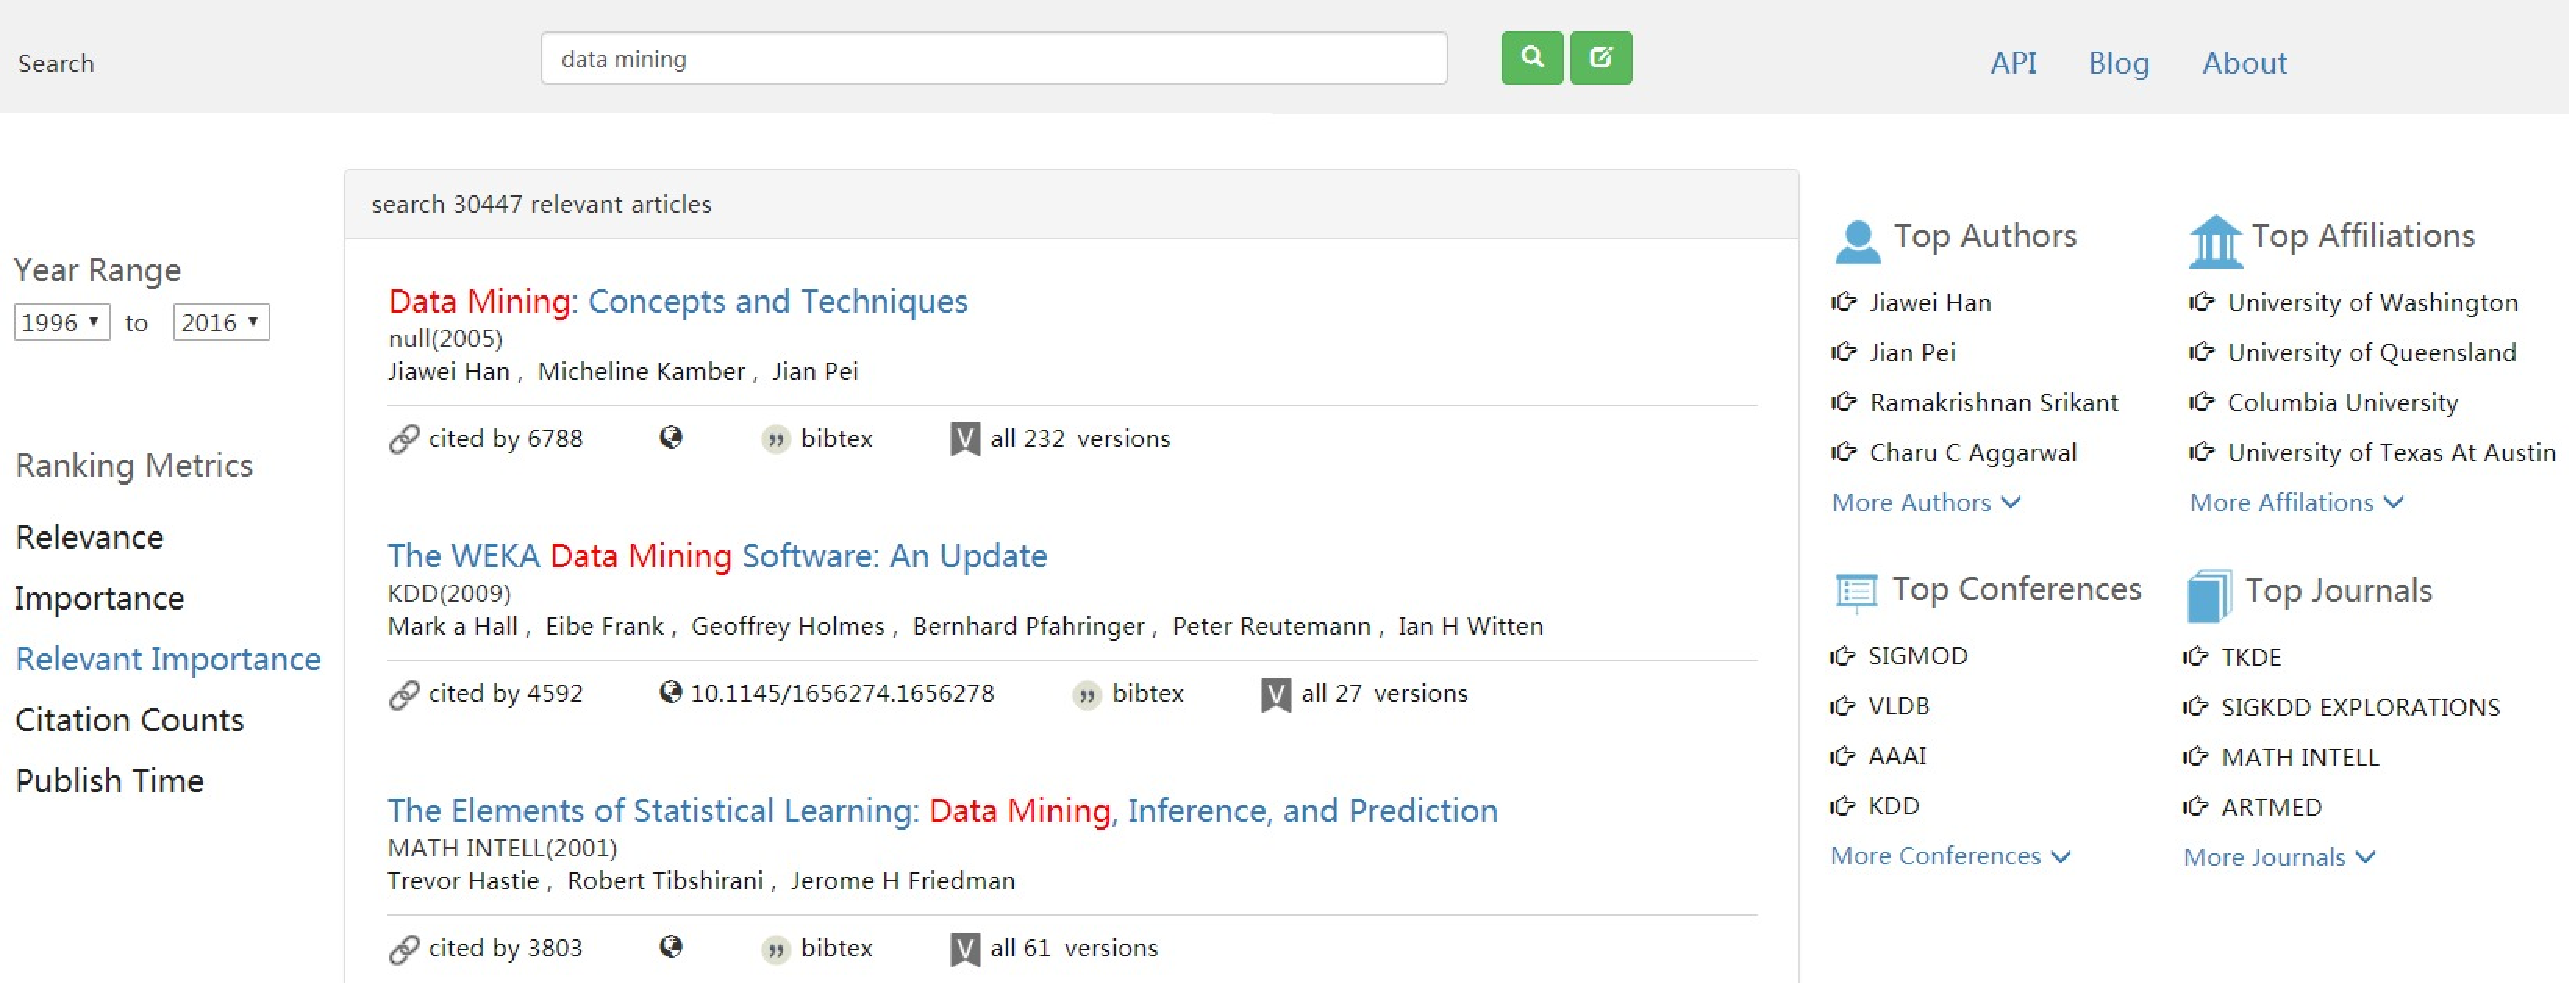
\includegraphics[width=\textwidth]{searchKeywords.pdf}
\caption{Heterogeneous entities ranking}
\label{fig:searchKeywords}
\vspace{-3ex}
\end{figure*}

\begin{figure}
\centering
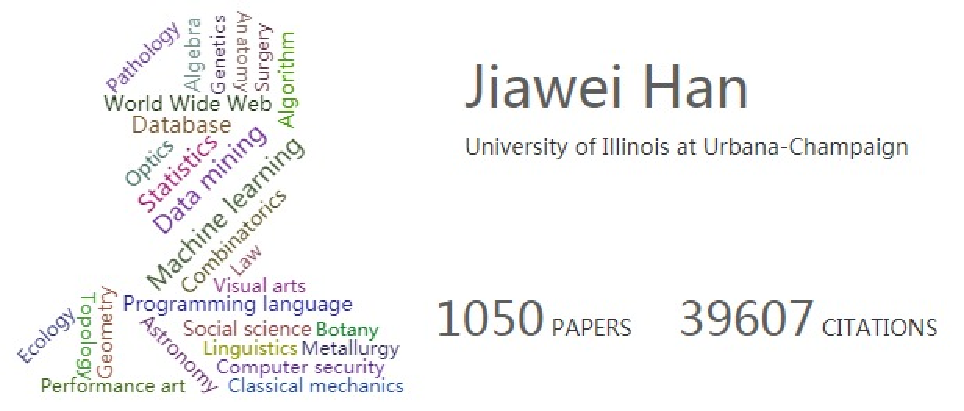
\includegraphics[width=0.8\columnwidth]{hjwAvatar.pdf}
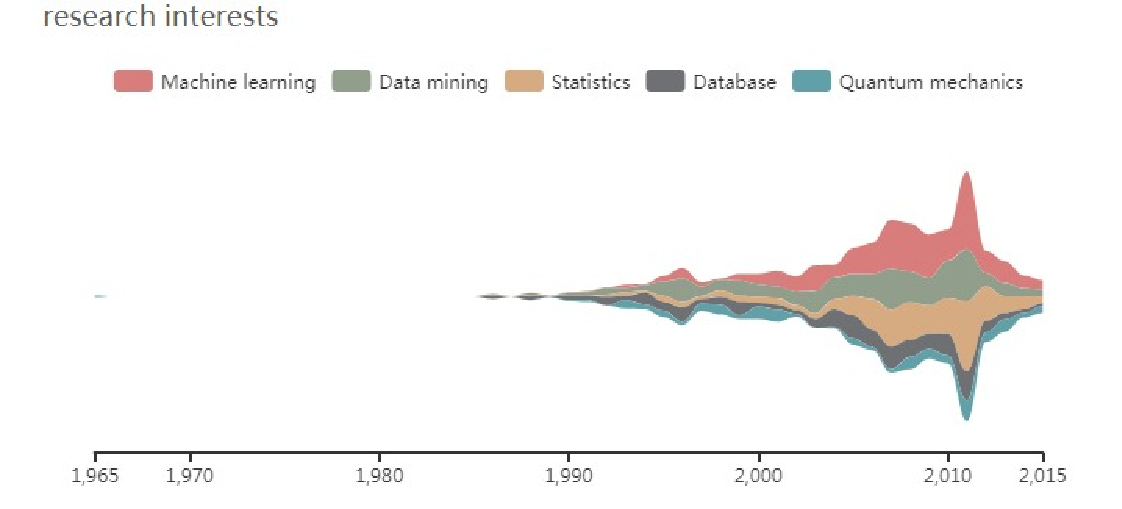
\includegraphics[width=0.8\columnwidth]{hjwInterest.pdf}
%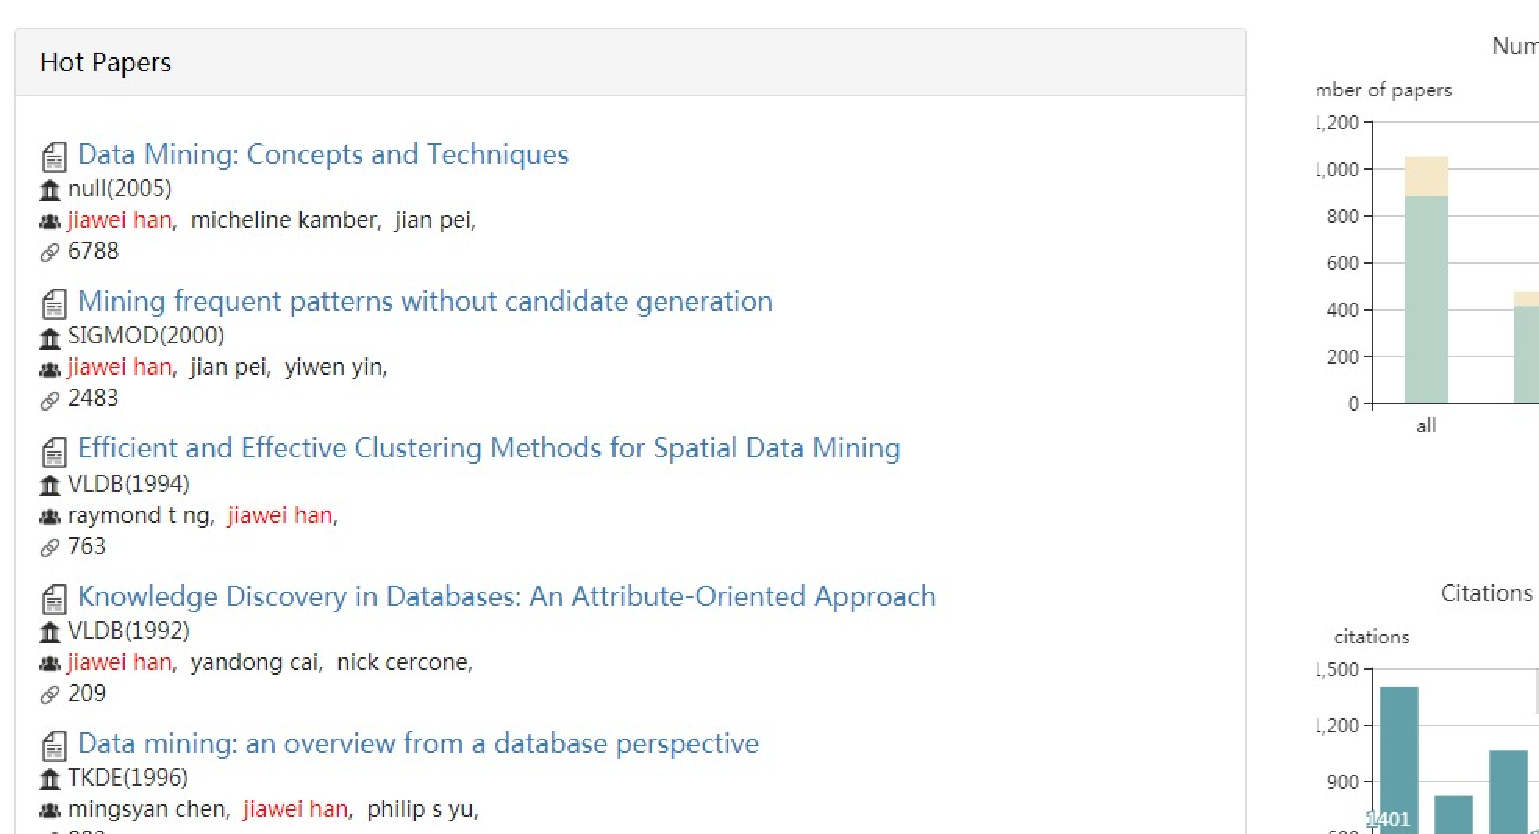
\includegraphics[width=\columnwidth]{hjwPapers.pdf}
\caption{Author profiling}
\label{fig:hjwProfile}
\vspace{-3ex}
\end{figure}

The demonstration consists of three parts: (1) We demonstrate heterogeneous entities ranking. (2) We give an example of author profiling. (3) We compare the query performance of Neo4j with MySQL.


%The demonstration consists of three parts. (1) We walk through its various ranking metrics to demonstrate the ability of \oursystem to query and rank heterogeneous entities. (2) To further illustrate the profiling function based on scholarly data analysis, we take author profiling as an example. (3) In the scholarly information search scenario, we compare the query performance of MySQL and Neo4j through experiments.

\stitle{Heterogeneous entities ranking.}
Consider a query ``graph database", the results are shown in Fig.~\ref{fig:searchKeywords}. The left side displays various ranking types and year range relevant to the keywords. And ranking type consists of {\em relevance}, {\em importance}, {\em relevant importance}, {\em citation} and {\em time}. 1-10 of 296 relevant papers are presented in the middle when users select {\em relevant importance}.
We also rank heterogeneous entities including, authors, affiliations, journals and conferences at the right. For example, ``Lei Chen", ``Mihalis Yannakakis", ``Jeffrey Xu Yu", ``M Tamer Ozsu" are selected as top authors in the field of ``graph database".
Moreover, \oursystem supports to query authors, affiliations, journals, conference series and conference instances in the search bar at the top.



\stitle{Author profiling.}
Fig.~\ref{fig:hjwProfile} is an example of author profiling. We demonstrate author's basic scholarly information including its institute, paper numbers and citations.
Author's avatar is described by word cloud and the weight of the each word is relevant to the important score of the article. As shown, ``machine learning" and ``data mining" are very clear in the avatar of Prof. Han.
Below the avatar we model the evolution of author's research interests through the statistics of publications' filed of study.
His publications keep growing before 2010, and the convex near 2011 is due to his numerous and influential publications such as ``data mining: concepts and techniques". More specifically, users are allowed to access relevant publications by clicking research interests. Author profiling also support to find co-authors, relevant affiliations, author's publications and statistics of its publications. However, we fail to display these due to space limitation.


\stitle{Query performance with Neo4j compared with MySQL.}
As shown in Table~\ref{tab-compare}, we test three query cases: search paper's title and authors by paper ID, search author��s top-10 papers by author ID and search top-10 cited papers by paper ID. Each query case has (2, 4, 3) {\em joins} in MySQL, respectively.
 All of query cases on Neo4j take less time than MySQL. More specifically, each of them improves the querying efficiency by (4.8\%, 52.8\%, 30.9\%). Thus, Neo4j with index-free adjacency is more efficient and cheaper than MySQL in handling complex joins.


\begin{table}[t!]
\begin{center}
\caption{Query performance with Neo4j compared with MySQL}
\label{tab-compare}
\begin{scriptsize}
\begin{tabular}{lp{2cm}p{2cm}p{2cm}}
\hline
{} & {search paper's title, author by pa.ID} & {search author's top-10 papers by au.ID} & {search top-10 cited papers by pa.ID}\\
\hline
MySQL & 0.251 s  & 6.493 s & 35.190 s \\
Neo4j & 0.239 s  & 3.062 s & 24.332 s \\
\hline
\end{tabular} \\ %\vspace{.5ex}
\end{scriptsize}
\end{center}
\end{table}


%\oursystem is equipped with both searching articles and querying other academic entities, \ie author, affiliation, journal, conference series and conference instance. Consider a query ``graph database", we present importance articles relevant to the keywords, {\em relevant importance} as default ranking metrics. \oursystem also supports {\em relevance}, {\em importance}, {\em citation} and {\em time} to fit various ranking scenarios, shown at the left of the Fig.~\ref{fig:searchKeywords}.
%\marked{ranking types, select relevant importance, xxx selected as top author.}

% articles were backed to front-end after Neo4j Query Engine executing the cypher.

%\par
%{\em Relevance} is more suitable for retrieving articles by keywords, because of the capture of  semantic-level relevance. {\em Importance} is more appropriate for discovering important articles of affiliations and venues. And {\em relevant importance} is a combination of the former, which aims to retrieve both relevant and important articles. {\em Time} gives appropriate order for newly published articles and {\em citation} helps to find most-cited articles. Moreover, we also demonstrate top-k authors, affiliations, journals/conferences corresponding to ranking metrics, shown at the right of Fig.~\ref{fig:searchKeywords}





%We demonstrate author profiling in \oursystem, which contains research interests, co-authors, relevant affiliations, author's publications and statistics of its publications.
%\marked{function, machine learning, data mining, coverage 2012}


%\par
%Fig. \ref{fig:hjwProfile} shows some information of author profiling. Author's avatar is described by word cloud and the weight of the each word is relevant to the important score of the article. We model the evolution of author's research interests through the statistics of publications' filed of study. More specifically, users are allowed to access relevant publications by clicking research interests. In this way, users are able to explore various scholarly information both broadly and deeply.
% profiling, word cloud according paper's importance score. avatar, research interest, also find author's paper according fos


%Fig. \ref{fig:hjwProfile} is an example of an Author Page, where contains author's basic information and author's detailed profiling. For basic information, users can check author's publications, related authors and author's affiliations. We also develop author's detailed profiling to have a knowledge of the author both from breadth and depth. Thus, we model the evolution of author's research interest, author's avatar with word cloud description, the statistics of publication, {\em etc}.


%In order to compare the performance with MySQL, We model a similar ER diagram based on the Neo4j schema. For many-to-many relationship we introduce an intermediate table and create index on it. All experiments were conducted on a machine with 2 Intel Xeon E5-2630 2.4GHz CPUs and 64 GB of Memory, running a 64 bit Windows 7 professional Ultimate system.
%\par
%As shown in Table \ref{tab-compare}, Neo4j improves the querying efficiency over (search article info, search author's top-k articles, top-k cited articles' info) by (4.8\%, 52.8\%, 30.9\%). Note that, each query case has (2, 4, 3) {\em joins} in MySQL, respectively. Thus, Neo4j with index-free adjacency is more efficient and cheaper than MySQL in handling complex joins.
%\marked{title. case, joins, performance index-free adjacency}


% native graph storage
% what, parameter. the result. why.
% will become the bottleneck
% Neo4j with native graph storage
% , more joins will


%All experiments were conducted on a machine with 2 Intel Xeon E5-2630 2.4GHz CPUs and 64 GB of Memory, running a 64 bit Windows 7 professional Ultimate system. And the disk cache was forbidden.
% moreover, A large number of indexes will also lead to a decrease in efficiency when updated database.




\eat{
\stitle{Ranking Instance} We rank the conference papers \eg SIGMOD following the metrics of {\em time ranking}. We only collect articles published earlier than 2016, so the top of {\em time ranking} is the maximum importance score in 2015. As shown in fig. \ref{fig:sigmod}, we put ``Spark SQL: Relational Data Processing in Spark" in second place, which has the most citations(653) in SIGMOD 2015 up to now. More generally, in our top 10, there are 3 articles that has the most citation in SIGMOD 2015.
% the description in ICDE 2018

\par
Although they share the same venue component in the same year, the author of the article has higher prestige and popularity, such as Matei Zaharia and Michael Armbrust. Besides, an article in VLDB cites the paper published in the same years that increases the prestige and popularity of the citation components. Thus, the paper possesses a higher importance score by assembling the component of citation, author and venue.
}

%\par
%\stitle{Affiliation profiling}. As shown in fig. \ref{}, we give an example of affiliation profiling. The layout of the Affiliation Page is similar with Search Page, users can discover publications using various ranking metrics and check statistics information, such as the importance author, relevant affiliation, famous journals/conferences.
%% affiliation profiling
%\par
%\stitle{Venue profiling} venue
